\documentclass[a4paper, 11pt]{article}
\usepackage{amsmath}
\usepackage{graphicx}
\usepackage{geometry}
\usepackage{listings}
\geometry{scale=0.8}
\linespread{1.5}
\usepackage{hyperref}
\usepackage{listings}
\usepackage{color}
\definecolor{dkgreen}{rgb}{0,0.6,0}
\definecolor{gray}{rgb}{0.5,0.5,0.5}
\definecolor{mauve}{rgb}{0.58,0,0.82}
\lstset{frame=shadowbox,
    language=lisp,
    aboveskip=3mm,
    belowskip=3mm,
    showstringspaces=false,
    columns=flexible,
    basicstyle={\small\ttfamily},
    keywordstyle=\color{blue},
    commentstyle=\color{dkgreen},
    stringstyle=\color{mauve},
    breaklines=true,
    breakatwhitespace=true,
    tabsize=3,
    numbers=left
}

\title{	
\normalfont \normalsize
\textsc{School of Data and Computer Science, Sun Yat-sen University} \\ [25pt] %textsc small capital letters
\rule{\textwidth}{0.5pt} \\[0.4cm] % Thin top horizontal rule
\huge  E07 FF Planner \\ % The assignment title
\rule{\textwidth}{2pt} \\[0.5cm] % Thick bottom horizontal rule
\author{17341203 Yixin Zhang}
\date{\normalsize\today}
}

\begin{document}
\maketitle
\tableofcontents
\newpage

\section{Examples}

\subsection{Spare Tire}
\label{sec:spare-tire}

\begin{lstlisting}[title=domain\_spare\_tire.pddl]
(define (domain spare_tire)
  (:requirements :strips :equality:typing)
  (:types physob location) 
  (:predicates  (Tire ?x - physob)
		(at ?x - physob ?y - location))

(:action Remove
             :parameters (?x - physob ?y - location)
             :precondition (At ?x ?y)
             :effect (and (not (At ?x ?y)) (At ?x Ground)))

  (:action PutOn
             :parameters (?x - physob)
             :precondition (and (Tire ?x) (At ?x Ground) 
                                (not (At Flat Axle)))
             :effect (and (not (At ?x Ground)) (At ?x Axle)))
  (:action LeaveOvernight
             :effect (and (not (At Spare Ground)) (not (At Spare Axle)) 
                          (not (At Spare Trunk)) (not (At Flat Ground)) 
                          (not (At Flat Axle)) (not (At Flat Trunk)) ))
 )

\end{lstlisting}
\begin{lstlisting}[title=spare\_tire.pddl]
(define (problem prob)
 (:domain spare_tire)
 (:objects Flat Spare -physob Axle Trunk Ground - location)
 (:init (Tire Flat)(Tire Spare)(At Flat Axle)(At Spare Trunk))
 (:goal (At Spare Axle))
)


\end{lstlisting}
\begin{figure}[h]
  \centering
  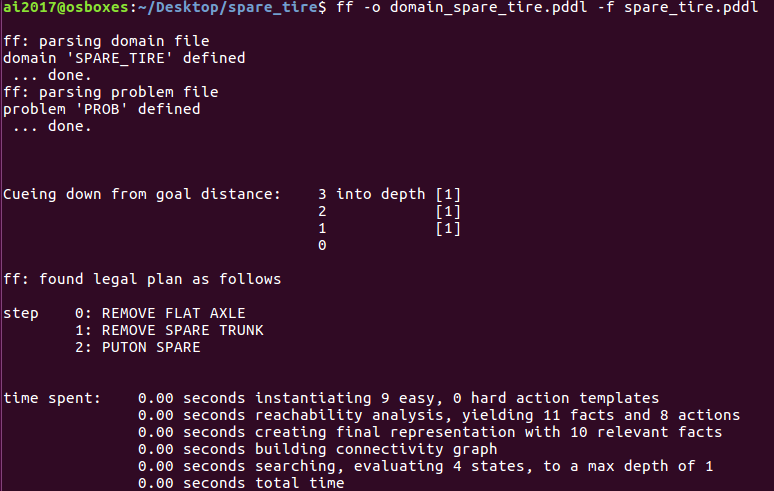
\includegraphics[width=16cm]{Pic/spare_tire}
\end{figure}

\subsection{Briefcase World}
\label{sec:briefcase-world}

Please refer to \texttt{pddl.pdf} at page 2. Please pay More attention to the usages of \texttt{forall} and \texttt{when}.  

For more examples, please refer to \texttt{ff-domains.tgz} and \texttt{benchmarksV1.1.zip}. For more usages of FF planner, please refer to the documentation \texttt{pddl.pdf}.
\section{Tasks}

\subsection{8-puzzle}
\begin{figure}[ht]
  \centering
  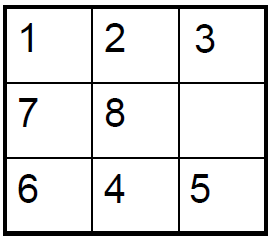
\includegraphics[width=0.4\textwidth]{Pic/puzzle}
  \qquad
  \parbox[b]{0.4\textwidth}{Please complete  \texttt{domain\_puzzle.pddl} and \texttt{puzzle.pddl} to solve the 8-puzzle problem.\\}
\end{figure}
\label{sec:8-puzzle}
\begin{lstlisting}[title=domain\_puzzle.pddl,frame=single,language=lisp,numbers=left]
(define (domain puzzle)
  (:requirements :strips :equality:typing)
  (:types num loc) 
  (:predicates  ())

(:action slide
             :parameters ()
             :precondition ()
             :effect () 
 )
)
\end{lstlisting}
\begin{lstlisting}[title=domain\_puzzle.pddl,frame=single,language=lisp,numbers=left]
(define (problem prob)
 (:domain puzzle)
 (:objects )
 (:init )
 (:goal ())
)

\end{lstlisting}
\subsection{Blocks World}
\label{sec:blocksworld}
\begin{figure}[h]
  \centering
  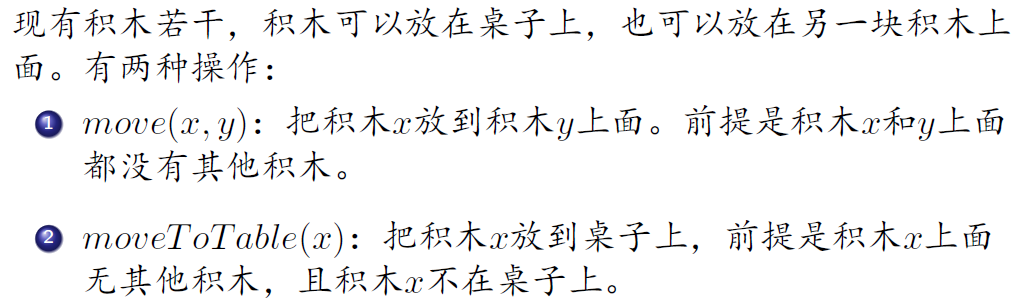
\includegraphics[width=17cm]{Pic/blocks}
\end{figure}

Please complete the file \texttt{domain\_blocks.pddl} to solve the blocks world problem. You should know the usages of \texttt{forall} and \texttt{when}.

\begin{lstlisting}[title=domain\_blocks.pddl,frame=single,language=lisp,numbers=left]
(define (domain blocks)
  (:requirements :strips :typing:equality
                 :universal-preconditions
                 :conditional-effects)
  (:types physob)
  (:predicates   
  	    (ontable ?x - physob)
            (clear ?x - physob)	
	    (on ?x ?y - physob))
		
  (:action move
             :parameters (?x ?y - physob)
             :precondition ()
             :effect ()
             )

  (:action moveToTable
             :parameters (?x - physob)
             :precondition ()
             :effect ( )
 )



\end{lstlisting}

\label{sec:problem-description}

\begin{lstlisting}[title=blocks.pddl]
(define (problem prob)
 (:domain blocks)
 (:objects A B C D E F - physob)
 (:init (clear A)(on A B)(on B C)(ontable C) (ontable D)
  (ontable F)(on E D)(clear E)(clear F)
)
 (:goal  (and (clear F) (on F A) (on A C) (ontable C)(clear E) (on E B) 
         (on B D) (ontable D)) )
 )
\end{lstlisting}

Please submit a file named \textsf{E07\_YourNumber.pdf}, and send it to \textsf{ai\_201901@foxmail.com}


\section{Codes and Results}

\subsection{8-puzzle}
\subsubsection{Overview}
I use nine number objects (num1 -- num8 and num0) to indicate the eight numbers and one empty cell, and nine location objects (loc1 -- loc8 and loc0) to indicate the nine cells on the puzzle, where locN is numN's target location.

When defining neighbourhood relationship, I just used one-way neighbour, i.e., I defined `neighbour loc1 loc2' without the existence of `neighbour loc2 loc1'. This works because I use `(or (neighbour ?from ?to) (neighbour ?to ?from))' to judge neighbourship. This won't be a problem.

\subsubsection{Code}
\begin{lstlisting}[title=domain\_puzzle.pddl]
(define (domain puzzle)
    (:requirements :strips :equality :typing)
    (:types number location)
    (:predicates
        (at ?n - number ?l - location)  ; indicates that the number `?n` is at location `?l`
        (neighbour ?l1 ?l2 - location)  ; indicates that `?l1` and `?l2` (or `?l2` and `?l1`) are neighbours
    )

    (:action slide  ; move the number `?num` from the cell `?from` to the cell `?to`
        :parameters (?num - number ?from ?to - location)
        :precondition (and
            (at ?num ?from)
            (at num0 ?to)
            (or (neighbour ?from ?to) (neighbour ?to ?from))
        )
        :effect (and
            (not (at num0 ?to))
            (at num0 ?from)
            (at ?num ?to)
        )
    )
)
\end{lstlisting}

\begin{lstlisting}[title=problem\_puzzle.pddl]
(define (problem prob)
    (:domain puzzle)
    
    (:objects
        loc1 loc2 loc3 loc4 loc5 loc6 loc7 loc8 loc0 - location  ; locN means numN's target location
        num1 num2 num3 num4 num5 num6 num7 num8 num0 - number    ; num0 indicates the empty cell
    )

    (:init
        ; initial configuration
        (at num1 loc1) (at num5 loc2) (at num2 loc3)
        (at num7 loc4) (at num4 loc5) (at num3 loc6)
        (at num8 loc7) (at num0 loc8) (at num6 loc0)

        ; define neighbourhoods (one-way neighbour is enough here)
        (neighbour loc1 loc2) (neighbour loc2 loc3)
        (neighbour loc4 loc5) (neighbour loc5 loc6)
        (neighbour loc7 loc8) (neighbour loc8 loc0)
        (neighbour loc1 loc4) (neighbour loc4 loc7)
        (neighbour loc2 loc5) (neighbour loc5 loc8)
        (neighbour loc3 loc6) (neighbour loc6 loc0)
    )

    (:goal (and
        (at num1 loc1) (at num2 loc2) (at num3 loc3)
        (at num4 loc4) (at num5 loc5) (at num6 loc6)
        (at num7 loc7) (at num8 loc8) (at num0 loc0)
    ))
)
\end{lstlisting}
\subsubsection{Result}
It works out correctly. For this simple example, the planner found a solution with eight steps, super cool.

\begin{figure}[h]
  \centering
  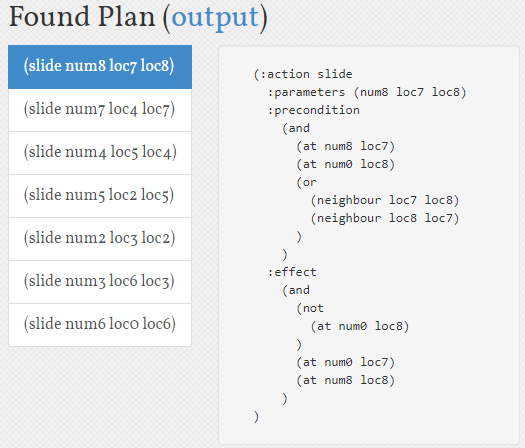
\includegraphics[width=13cm]{Pic/puzzlepddlresult.png}
\end{figure}

\begin{figure}[h]
  \centering
  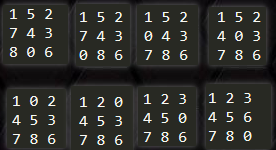
\includegraphics[width=10cm]{Pic/puzzleresult.png}
\end{figure}

\subsection{Blocks World}
\subsubsection{Overview}
Remember to manage the state of the block under x carefully after moving x away! Here, `forall` and `when` statements are used.

\subsubsection{Code}
\begin{lstlisting}[title=domain\_blocks.pddl]
(define (domain blocks)
    (:requirements :strips :typing :equality :universal-preconditions :conditional-effects)
    (:types physob)  ; physical object

    (:predicates
        (ontable ?x - physob)  ; block `?x` is on the table
        (clear ?x - physob)    ; there is no block on top of `?x`
        (on ?x ?y - physob)    ; `?x` is on top of `?y`
    )

    (:action move  ; move `?x` to top of `?y`
        :parameters (?x ?y - physob)
        :precondition (and (clear ?x) (clear ?y) (not (= ?x ?y)))
        :effect (and
            (forall (?z - physob) (when (on ?x ?z) (and (clear ?z) (not (on ?x ?z)))))
            (on ?x ?y) (not (clear ?y))
        )
    )

    (:action moveToTable  ; move `?x` to the table
        :parameters (?x - physob)
        :precondition (and (clear ?x) (not (ontable ?x)))
        :effect (and
            (forall (?z - physob) (when (on ?x ?z) (and (clear ?z) (not (on ?x ?z)))))
            (ontable ?x)
        )
    )
)
\end{lstlisting}

\begin{lstlisting}[title=problem\_blocks.pddl]
(define (problem prob)
    (:domain blocks)

    (:objects A B C D E F - physob)

    (:init
        (clear A) (on A B) (on B C) (ontable C)
        (clear E) (on E D) (ontable D)        
        (clear F) (ontable F)
    )

    (:goal (and
        (clear F) (on F A) (on A C) (ontable C)
        (clear E) (on E B) (on B D) (ontable D)
    ))
)
\end{lstlisting}

\subsubsection{Result}
\begin{figure}[h]
  \centering
  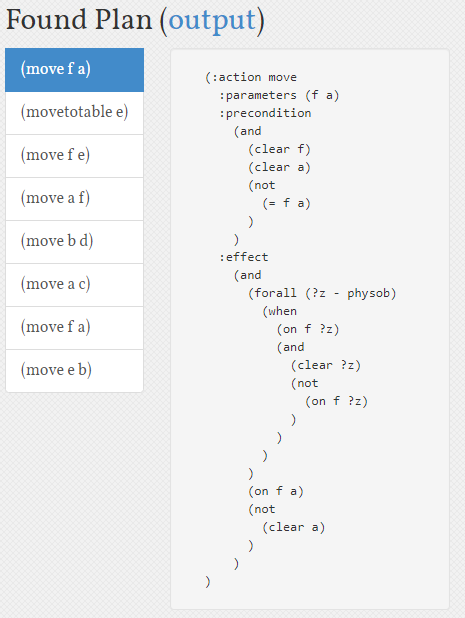
\includegraphics[width=13cm]{Pic/blocksresult.png}
\end{figure}




%\clearpage
%\bibliography{E:/Papers/LiuLab}
%\bibliographystyle{apalike}
\end{document} 
%%% Local Variables:
%%% mode: latex
%%% TeX-master: t
%%% End:
